\section{Implementação do Algoritmo Rocket}
\label{sec:7.3}

No Rocket, a execução do algoritmo genético ocorre a partir de uma requisição que concentra os dados acadêmicos necessários à geração da grade horária, contendo informações sobre disponibilidades docentes, matrizes curriculares, turmas, vínculos entre professores e disciplinas, parâmetros do algoritmo genético, parâmetros da função \textit{fitness} e, quando necessário, uma URL de callback para envio do resultado.

Antes de iniciar a evolução, o Rocket organiza os dados recebidos por meio da construção de índices auxiliares, criando mapas de acesso rápido para disponibilidades, matrizes, turmas, professores, dias da semana, turnos e vínculos. Entre essas estruturas, destaca-se a lista de candidatos, que armazena para cada matriz curricular quais disponibilidades podem ser utilizadas, considerando o turno da turma e o vínculo entre professor e disciplina.

A representação genética do Rocket difere da utilizada no Sunny e no Morpheus. Enquanto nesses o gene é representado por um par explícito entre matriz e disponibilidade, no Rocket o gene é armazenado como um único valor inteiro correspondente ao identificador de uma disponibilidade. A posição desse gene dentro do cromossomo possui significado próprio: a implementação mantém uma lista ordenada de matrizes, e cada posição do vetor de genes corresponde a uma matriz específica. O valor presente naquela posição indica qual disponibilidade foi atribuída à matriz correspondente. Genes sem alocação recebem o valor unallocatedID = 0.

A população inicial é gerada a partir dos candidatos previamente definidos para cada matriz. Essa geração pode ser classificada como uma inicialização híbrida: a escolha final é aleatória, mas ocorre preferencialmente dentro de um subconjunto menos propenso a conflitos. Quando há alternativas livres para a turma, o sorteio ocorre entre essas opções; quando não há, entre todos os candidatos disponíveis. Um aspecto técnico importante é que a geração da população inicial pode ser paralelizada por meio de \textit{goroutines}, melhorando o desempenho operacional em execuções com populações maiores.

A função \textit{fitness} do Rocket calcula uma pontuação inicial a partir do número total de genes multiplicado pela pontuação base, cujo valor padrão é 10. Além disso, cada alocação válida recebe um bônus adicional de 2 pontos (validBonus) e é aplicado um bônus de diversidade de 5 pontos (diversityBonus) para cada matriz adicional atribuída ao mesmo professor. As penalidades são os elementos mais decisivos: conflito de professor possui o maior peso, com penalidade padrão de 12.000 pontos, refletindo que um docente não pode ministrar duas aulas simultaneamente; conflito de turma recebe penalidade de 8.000 pontos; genes não alocados recebem 10.000 pontos; e dados inválidos ou incompletos também recebem 10.000 pontos. Os pesos são configuráveis por meio dos parâmetros da requisição.

A seleção por torneio cria pressão seletiva moderada. O \textit{crossover} utilizado é de um ponto, implementado de modo que dois pais gerem um novo filho: o algoritmo sorteia um ponto de corte e os genes anteriores a esse ponto são herdados do primeiro pai, enquanto os posteriores são herdados do segundo. A mutação é aplicada gene a gene, selecionando a nova disponibilidade dentro da lista de candidatos válidos para a matriz correspondente.

O reparo do Rocket é implementado como uma tentativa ativa de realocação. O algoritmo calcula ocupações de professor e turma, identifica genes associados a conflitos ou ausência de alocação, e busca a melhor alternativa possível dentro do conjunto de candidatos. A escolha da nova disponibilidade é orientada por uma pontuação interna de conflito: candidatos que colidem com a agenda do professor recebem acréscimo maior, enquanto candidatos que colidem com a agenda da turma recebem acréscimo menor. O algoritmo escolhe o candidato com menor pontuação.

O critério de parada do Rocket combina um limite fixo de gerações com mecanismos de parada antecipada. A execução pode ser interrompida quando uma solução sem erros é encontrada, isto é, quando a melhor grade da geração possui quantidade total de erros igual a zero. Na implementação, esse total corresponde à soma entre disciplinas não alocadas, conflitos de professor, conflitos de turma e dados inválidos ou incompletos. Quando essa condição ocorre, a geração da solução sem erros é registrada e o processo evolutivo é encerrado imediatamente.

Além disso, o Rocket interrompe a evolução quando passa muitas gerações sem melhorar a melhor \textit{fitness} global. O limite de gerações sem melhoria é calculado como 20\% do total de gerações configurado, respeitando um mínimo de 25 e um máximo de 200 gerações, conforme a expressão \texttt{max(25, min(200, numeroGeracoes * 0.20))}. Assim, para 100 gerações configuradas, o limite sem melhoria é 25; para 1.000 gerações, é 200; e para 2.000 gerações, permanece em 200. A melhora considerada nesse critério é uma melhora de \textit{fitness}, não apenas uma redução direta da quantidade de erros. Caso a diferença entre a geração atual e a última geração com melhora alcance esse limite, a execução é interrompida e a resposta indica parada antecipada.

Por fim, se nenhuma das condições anteriores for satisfeita, o algoritmo continua até atingir o número máximo de gerações configurado. O valor padrão utilizado pelo Rocket é de 1.000 gerações, podendo ser sobrescrito na requisição por meio do parâmetro \texttt{numeroGeracoes}. Ao final, o melhor cromossomo é decodificado em uma grade horária e as métricas finais são calculadas, contabilizando disciplinas não alocadas, conflitos de professor, conflitos de turma e dados incompletos, gerando também mensagens textuais de conflito para integração com outros sistemas.

\begin{figure}[H]
\centering
\caption{Fluxo de execução do algoritmo genético Rocket}
\label{fig:fluxo-rocket}

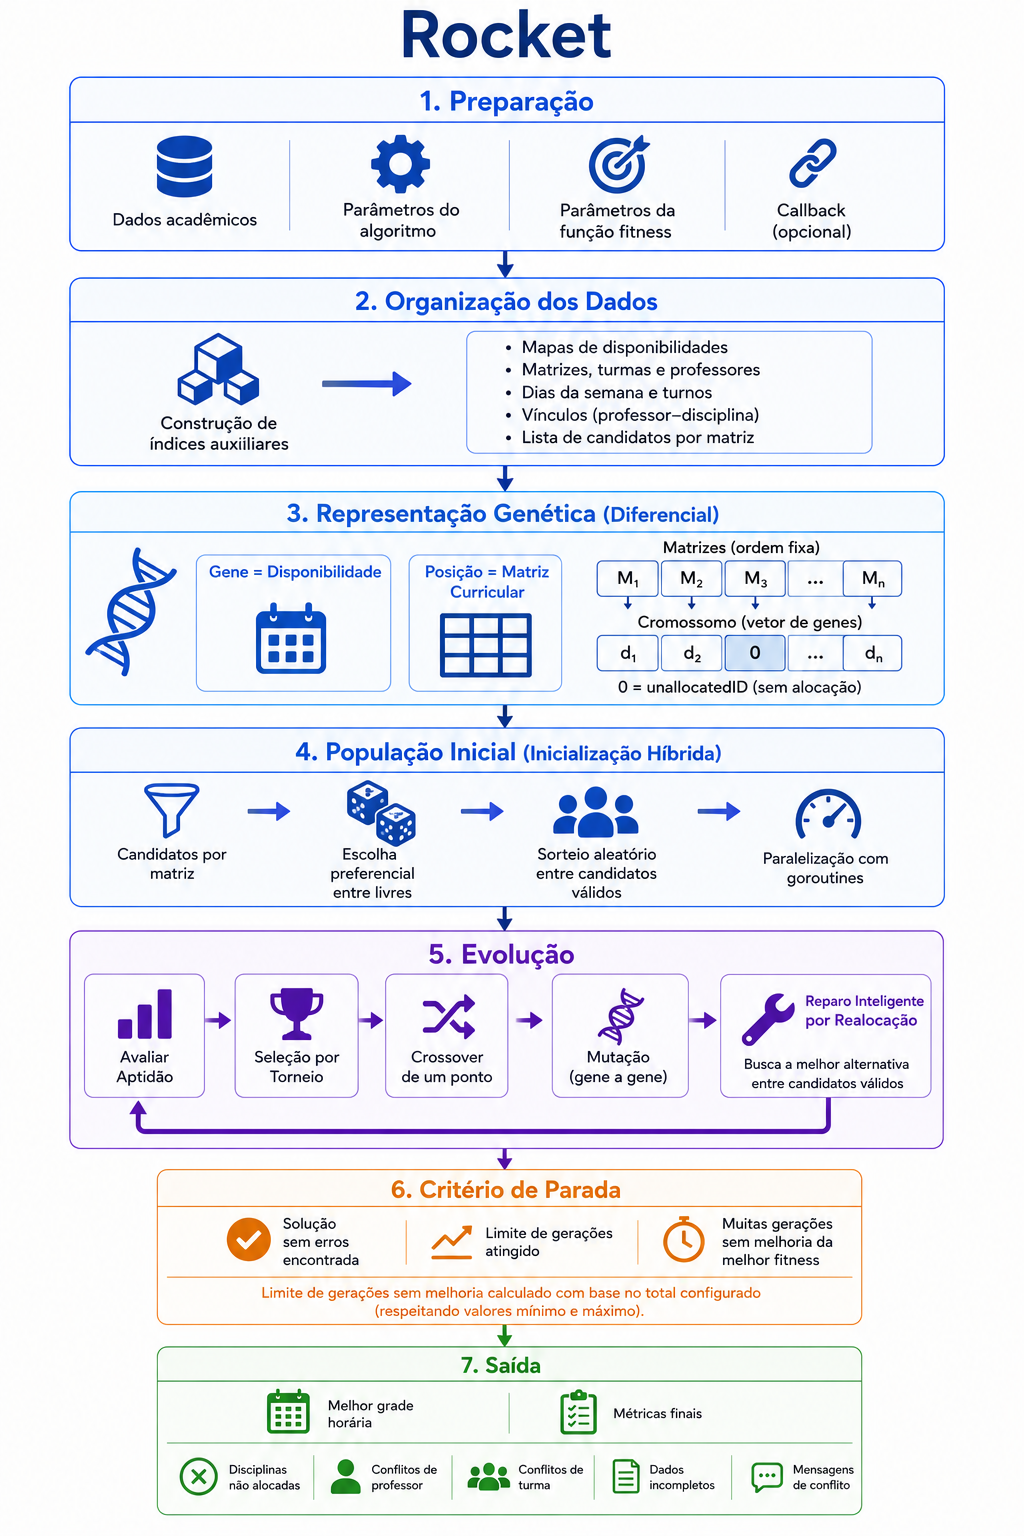
\includegraphics[width=0.85\textwidth]{figuras/Figura_17_ilustracaoFluxoRocket.png}

\vspace{0.2cm}
\fonteautores
\end{figure}
